
\documentclass[conference]{IEEEtran}
\usepackage{amsmath}
\usepackage{amssymb}
\usepackage{graphicx}
\usepackage{cite}
\usepackage{url}
\usepackage{algorithm}
\usepackage{algorithmic}
\usepackage{booktabs}
\usepackage{multirow}
\usepackage{hyperref}
\graphicspath{{figures/}}

\begin{document}

\title{Cheap Structured Memory for LLM Agents: A Cost--Retention Study on Real Long-Conversation Benchmarks}

\author{\IEEEauthorblockN{Ishan Gautam}
\IEEEauthorblockA{
\textit{Pulchowk Campus} \\
\textit{Institute of Engineering, Tribhuvan University} \\
Lalitpur, Nepal \\
080bct034.ishan@pcampus.edu.np
}
\and
\IEEEauthorblockN{Kushal K.C.}
\IEEEauthorblockA{
\textit{Pulchowk Campus} \\
\textit{Institute of Engineering, Tribhuvan University} \\
Lalitpur, Nepal \\
080bct041.kushal@pcampus.edu.np
}
}

\maketitle

\begin{abstract}
Large language model (LLM) agents incur token costs that grow super-linearly with conversation length because each step may re-send an expanding history. Persistent external memory is often proposed as a remedy, but its retention/cost trade-off is easy to overstate and is frequently measured only on short or synthetic data. This paper studies cheap-extractor structured memory for LLM agents---a small model extracts durable facts from conversation segments into latest-value subject--predicate \emph{slots}, optionally combined with sparse retrieval over past turns, and a larger model answers from that compact memory plus a recent-message window---and evaluates it on \emph{real, human-annotated long-conversation benchmarks} rather than self-generated data. Using the LoCoMo benchmark (multi-session conversations of 369--680 turns) with an LLM-as-judge protocol, we compare seven strategies: full context, truncation, running summary, append-only notes, fact slots, BM25 retrieval, and a slots+retrieval hybrid. On $n=160$ human-written questions, BM25 retrieval and the slots+retrieval hybrid cut real input tokens by over 96\% and cost to 5--9\% of full context while \emph{not losing} retention---their point estimates are above full context (39.4\% and 38.8\% vs. 30.6\%) and a question-level paired sign test shows only a non-significant \emph{trend} in their favor ($p=0.09$ and $0.12$); a power analysis indicates $\approx$360--430 questions would be needed to confirm an advantage of this size. Against truncation, however, both are significantly better ($p<0.001$). We add a per-category breakdown and an error analysis showing that sparse retrieval recovers only $\sim$13\% of the gold evidence turns on multi-hop questions (explaining where it fails). A LongMemEval evaluation across knowledge-update ($n=72$) and the temporal, multi-session, and abstention categories ($n=135$) confirms the same ordering: retrieval and the slots+retrieval hybrid match full context while fact slots alone are consistently the weakest method. We position BM25 retrieval as the strongest single cost/retention lever; latest-value fact slots are the weakest method on both general QA and their intended knowledge-update use-case, because a cheap extractor misses most fact updates. We also document a concrete operational finding: on a free inference tier, full-context prompting of real long conversations is rejected above a per-request token cap, whereas compact-memory methods run unimpeded. We release the harness, the real-benchmark adapters, the judge, and per-question results.
\end{abstract}

\begin{IEEEkeywords}
large language model agents, long-term memory, LLM cost optimization, LoCoMo, LongMemEval, retrieval-augmented generation, fact-slot memory, model cascading, token-efficient prompting, conversational memory benchmarks, LLM-as-judge, agentic systems
\end{IEEEkeywords}

\section{Introduction}

Autonomous AI agents have revolutionized tasks ranging from market intelligence to sales outreach, yet their economic viability remains challenged by escalating token costs. Unlike traditional chat applications where a single query consumes approximately 1,000 tokens, autonomous agents perform multi-step reasoning, tool calls, and context re-stacking, consuming 20,000 to 100,000 tokens minimum per task \cite{zhou2024agents, park2023generative}.

The problem intensifies as conversations lengthen. As agents carry more history behind each step, the cumulative token cost over a multi-turn task grows quadratically rather than linearly. Poorly architected agents can consume resources at unsustainable rates once realistic retry rates, parallel instances, and tool overhead are accounted for \cite{shinn2023reflexion}. Worse, simply enlarging the context window is not a free remedy: long-context models exhibit a ``lost in the middle'' effect, where information placed away from the beginning or end of a long prompt is poorly utilized \cite{nfliu2023lost}, and the self-attention mechanism makes each additional token quadratically expensive in compute \cite{packer2023memgpt}.

Current mitigation strategies include:
\begin{enumerate}
    \item \textbf{Semantic Caching}: Reuse outputs for semantically similar inputs \cite{bang2023gptcache}.
    \item \textbf{History Summarization}: Compress past conversations into running summaries to bound context length \cite{acl2024}.
    \item \textbf{Model Cascading}: Use small models for easy sub-tasks and escalate to expensive models only when required \cite{chen2023frugalgpt}.
    \item \textbf{Prompt Compression}: Drop low-information tokens before inference using a small scoring model \cite{jiang2023llmlingua}.
    \item \textbf{Hierarchical / Virtual Memory}: Page information in and out of the context window from external storage \cite{packer2023memgpt}.
\end{enumerate}

However, existing approaches face limitations. Naive truncation discards critical information indiscriminately. Aggressive summarization may drop important details \cite{acl2024}. Semantic caching only helps when queries repeat. Prompt compression operates at the token level and does not produce a durable, queryable record of the conversation. Crucially, most summarization implementations use the \emph{same} expensive model for both compression and synthesis, leaving the largest cost-saving lever -- a cheap extractor -- untouched. Prior work on agent memory highlights the need for structured, persistent approaches beyond simple summarization \cite{park2023generative, zhong2024memorybank, zhang2024memorysurvey}.

\textbf{Our Contribution}: This paper proposes and stress-tests a \textit{hierarchical Fact-Slot memory architecture} that combines model cascading with structured history summarization. A small model extracts durable facts from conversation segments, upserts them into a persistent latest-value slot table, and subsequent prompts reference this compact table alongside only recent messages. Concretely, this paper makes the following contributions:
\begin{enumerate}
    \item A token-cost model that makes explicit why full-context agents scale quadratically over a multi-turn task, and a retention requirement that formalizes the information an agent must preserve (Section~\ref{sec:problem}).
    \item A persistent memory architecture that applies the model-cascading insight to the \emph{memory} step -- a cheap extractor writes latest-value fact slots, an expensive model only synthesizes -- together with concrete schemas and extraction prompts (Section~\ref{sec:method}).
    \item An evaluation protocol -- metrics, seven baselines, an LLM-as-judge scorer, and adapters to the real LoCoMo and LongMemEval benchmarks -- for measuring token reduction, cost, and per-category retention with question-level paired statistics (Section~\ref{sec:experiments}).
    \item An open-source reference implementation released as a research repository (Section~\ref{sec:implementation}).
\end{enumerate}
We evaluate on real, human-annotated long conversations rather than self-generated data. The result reverses an earlier short, synthetic pilot: at realistic conversation lengths, sparse retrieval and a slots+retrieval hybrid match or exceed full-context retention while costing 5--10\% as much, with the largest gains on single-hop, open-domain, and temporal questions and a remaining full-context advantage on multi-hop reasoning. A dedicated LongMemEval knowledge-update evaluation ($n=72$) confirms the same ordering: BM25 retrieval matches full context (73.6\% vs.\ 69.4\%), while fact slots alone are worst (37.5\%), showing that the extractor bottleneck dominates the representational advantage of slot-based memory. The same holds across LongMemEval's temporal, multi-session, and abstention categories ($n=135$), where the slots+retrieval hybrid matches full context (45.2\%) and fact slots remain the weakest method (15.6\%).

\section{Related Work}

Memory optimization for LLM agents has emerged as a critical research area; a recent survey systematizes the design space of agent memory across short-term context, long-term storage, and the read/write mechanisms that connect them \cite{zhang2024memorysurvey}. We position our contribution within three adjacent lines of work: prompt compression, model cascading, and persistent agent memory.

\textbf{Prompt and context compression.} LLMLingua uses a small language model to score and remove low-information tokens from a prompt in a coarse-to-fine manner, achieving up to $20\times$ compression with limited performance loss \cite{jiang2023llmlingua}. This validates the central premise that a cheap model can identify what matters, but compression is ephemeral -- it rewrites a single prompt and leaves no reusable record of the conversation. The motivation for compression is reinforced by evidence that models do not use long contexts uniformly: relevant content placed in the middle of a long prompt is systematically underused \cite{nfliu2023lost}.

\textbf{Model cascading.} FrugalGPT demonstrates that routing queries through a cascade of progressively more expensive models can match GPT-4 quality at up to 98 percent lower cost \cite{chen2023frugalgpt}. Cascading is highly effective for answering, but prior cascades target the \emph{response} step rather than the \emph{memory} step; they do not use the cheap model to maintain long-term state. Our work applies the cascade insight specifically to extraction-and-storage.

\textbf{Persistent agent memory.} Park et al. introduce Generative Agents, whose memory stream and retrieval support coherent long-horizon behavior, but their focus is believable simulation rather than cost \cite{park2023generative}. Zhong et al. propose MemoryBank, a dynamic memory-updating mechanism for LLMs that shares our persistence goal but uses a single model and does not exploit cascading \cite{zhong2024memorybank}. MemGPT frames the context window as virtual memory, paging information between an in-context tier and external storage via function calls \cite{packer2023memgpt}; our fact-slot table is a deliberately simpler realization of the same external-memory idea, with the added emphasis that writes are performed by a cheaper model. Recent conversation-summarization systems combine recent dialogue with a running summary of earlier turns \cite{acl2024}, but typically employ a single model without separating cheap extraction from expensive synthesis. Our work bridges these gaps by combining structured extraction by a small model, persistent latest-value storage, and selective context retrieval with explicit overwrites for updated facts.

\section{Problem Formulation}
\label{sec:problem}

\subsection{Token Cost Growth Model}

Let $C(n)$ denote the token cost for a conversation with $n$ messages. In traditional approaches where full history is retained:

\begin{equation}
C(n) = \alpha_{\text{large}} \cdot \sum_{i=1}^{n} \text{tokens}(m_i) + \beta_{\text{large}} \cdot \text{tokens}(m_{\text{out}})
\end{equation}

where $\alpha_{\text{large}}$ represents the input cost per token for the large model (typically \$0.003 to \$0.005 per 1,000 tokens), $\beta_{\text{large}}$ represents the output cost per token, $m_i$ denotes the $i$-th message, and $m_{\text{out}}$ represents the generated response.

Since $\sum_{i=1}^{n} \text{tokens}(m_i)$ grows linearly with $n$, and each API call includes this cumulative context, the total cost for $k$ conversation turns grows approximately as:

\begin{equation}
\text{Total Cost}_{\text{full}}(k) \approx \sum_{j=1}^{k} C(j) \propto k^2
\end{equation}

For example, if each turn adds roughly $b$ input tokens and output length is treated as a lower-order term, then $C(j) \approx \alpha_{\text{large}} b j$ and
\begin{equation}
\sum_{j=1}^{k} C(j) \approx \alpha_{\text{large}} b \frac{k(k+1)}{2} = O(k^2).
\end{equation}

For our hierarchical approach, the cost includes both synthesis (large model) and maintenance (small model extraction):

\begin{multline}
\text{Total Cost}_{\text{hier}}(k) = \\
\underbrace{\textstyle\sum_{j=1}^{k} \alpha_{\text{large}} (\text{tokens}(\mathcal{F}_j) + \text{tokens}(M_{\text{recent}}))}_{\text{synthesis}} \\
+ \underbrace{\textstyle\sum_{s=1}^{S} \alpha_{\text{small}} \cdot \text{tokens}(\text{segment}_s)}_{\text{extraction}}
\end{multline}

where $\mathcal{F}_j$ is the current fact-slot table at turn $j$, $M_{\text{recent}}$ is the recent message window, $S$ is the number of extraction calls, and $\alpha_{\text{small}} \ll \alpha_{\text{large}}$. This expression yields a cost advantage only if $\mathcal{F}_j$ is kept smaller than the raw transcript; append-only memory can still grow enough to erase the expected savings at short horizons, while latest-value slots bound repeated subject--predicate facts.

\subsection{Information Retention Requirement}

An agent must maintain access to $I_{\text{critical}}$, the set of critical information entities from conversation history. Let $\mathcal{S} \subseteq \text{History}$ denote the subset retained in context. The system requires:

\begin{equation}
\text{Retention}(\mathcal{S}) = \frac{|I_{\text{critical}} \cap \mathcal{S}|}{|I_{\text{critical}}|} \geq \theta
\end{equation}

where $\theta$ represents the minimum acceptable retention threshold (typically $\theta \geq 0.9$ for reliable task completion).

\section{Proposed Method}
\label{sec:method}

\subsection{Architecture Overview}

Our hierarchical memory system comprises three components operating in sequence:

\begin{figure}[t]
\centering
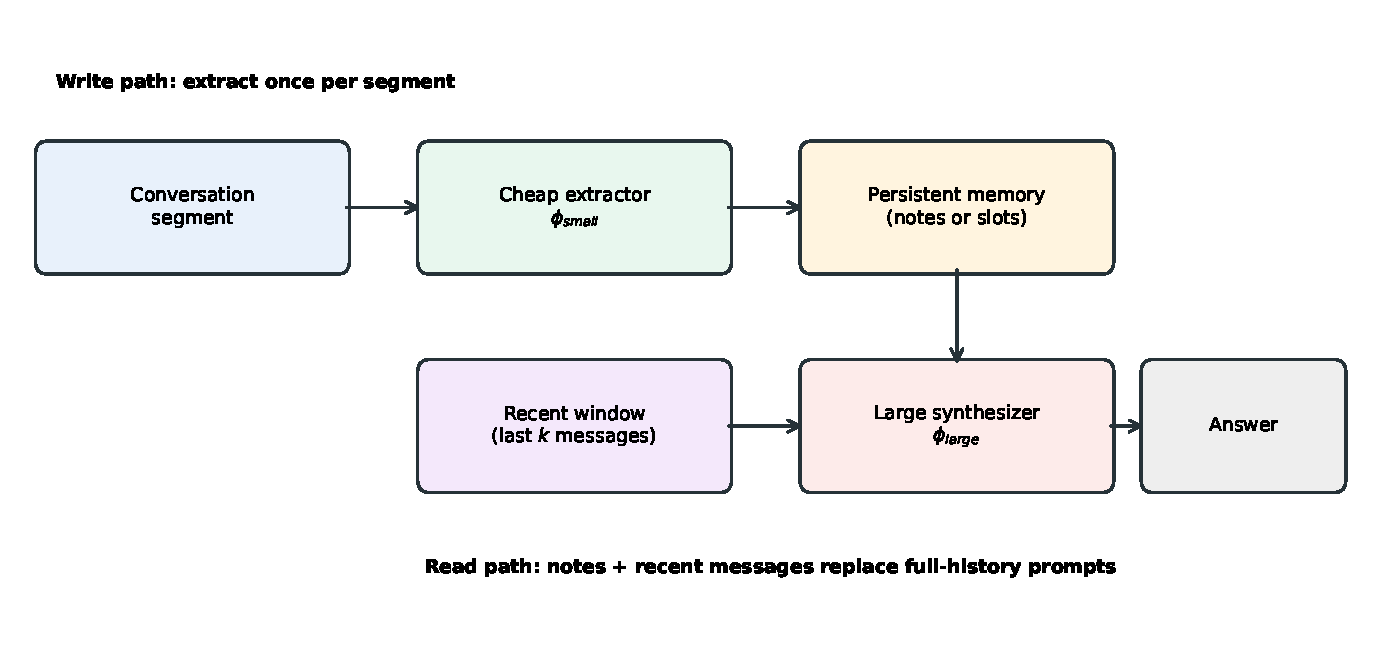
\includegraphics[width=\columnwidth]{architecture_flowchart.pdf}
\caption{Hierarchical fact-slot memory architecture: a cheap extractor writes latest-value fact slots, and a large synthesizer answers from the slot table plus a recent-message window.}
\label{fig:architecture}
\end{figure}

\begin{algorithm}[ht]
\caption{Fact-Slot Conversation Management}
\label{alg:hierarchical}
\begin{algorithmic}[1]
\REQUIRE Conversation segment $M = \{m_1, \dots, m_k\}$, fact-slot table $\mathcal{F}$
\ENSURE Updated slot table $\mathcal{F}'$, Response $r$
\STATE $\text{slots} \gets \phi_{\text{small}}(M, \text{prompt}_{\text{slot}})$ \COMMENT{Extract subject--predicate facts}
\STATE $\mathcal{F}' \gets \text{upsert}(\mathcal{F}, \text{slots})$ \COMMENT{Overwrite by latest timestamp}
\STATE $\text{context} \gets \text{concat}(\mathcal{F}', M_{\text{recent}})$ \COMMENT{Build compressed context}
\STATE $r \gets \phi_{\text{large}}(\text{context}, \text{prompt}_{\text{synthesis}})$ \COMMENT{Generate response}
\RETURN $\mathcal{F}', r$
\end{algorithmic}
\end{algorithm}

\subsection{Small Model Extraction}

The slot extraction prompt $\text{prompt}_{\text{slot}}$ instructs $\phi_{\text{small}}$ to identify durable facts as latest-value slots:

\begin{equation}
\begin{split}
\text{slot} = (\,&\text{subject},\ \text{predicate},\ \text{value},\\
&\text{timestamp},\ \text{evidence}\,)
\end{split}
\end{equation}

Example extraction prompt:
\begin{quote}
From the following conversation, extract durable fact slots. Return JSON with key \texttt{facts}, where each fact has \texttt{subject}, \texttt{predicate}, \texttt{value}, and \texttt{evidence}. If a segment corrects a fact, emit the corrected current value.
\end{quote}

\subsection{Fact-Slot Table Format}
\label{sec:slot-format}

Fact-Slot Memory stores durable facts in a latest-value table rather than an append-only summary. Each extracted fact is normalized as

\begin{equation}
f_t = (\text{subject}, \text{predicate}, \text{value}, \text{timestamp}, \text{evidence}).
\end{equation}

The memory table $\mathcal{F}$ is keyed by $(\text{subject}, \text{predicate})$:

\begin{equation}
\mathcal{F}[\text{subject}, \text{predicate}] = (\text{value}, \text{timestamp}, \text{evidence}).
\end{equation}

When a later segment states a new value for the same key, the system overwrites the old value while keeping a lightweight event log for reproducibility. At read time, the prompt contains only the current slot table plus the recent window. This representation is less general than free-form notes, but it is better matched to fact-tracking conversations with updates such as changed dates, owners, budgets, or priorities. It also provides an explicit mechanism for resolving contradictions by timestamp, a failure mode of append-only notes.

\subsection{Append-only Notes Baseline}
\label{sec:notes-format}

For comparison, we also evaluate the earlier append-only JSON notes representation. It stores extracted entities, decisions, facts, goals, and action items for each segment without overwriting old values. This baseline is useful for isolating the effect of the Fact-Slot representation: append-only notes preserve more historical context, but they can grow quickly and retain obsolete facts.

\subsection{Model Selection}

The architecture is model-agnostic, but the empirical results in this paper use a specific Groq-hosted Llama cascade:
\begin{itemize}
    \item \textbf{Small extractor} ($\phi_{\text{small}}$): \texttt{llama-3.1-8b-instant}
    \item \textbf{Large synthesizer} ($\phi_{\text{large}}$): \texttt{llama-3.3-70b-versatile}
\end{itemize}

More generally, the intended configuration is a cheaper extractor paired with a more capable synthesizer, analogous to model-cascade systems such as FrugalGPT \cite{chen2023frugalgpt}. A favorable price ratio is necessary but not sufficient: the Fact-Slot representation must also retain the facts needed for downstream answering and remain small enough to offset extractor maintenance.

\section{Experimental Design}
\label{sec:experiments}

\subsection{Datasets}
\label{sec:datasets}

We evaluate on two openly released, human-annotated long-conversation memory
benchmarks rather than on self-generated data. This directly addresses the main
threat to validity of an earlier synthetic pilot (planted-fact strings over
short dialogues): the conversations here are multi-session, span hundreds of
turns, and the questions were written and verified by humans.

\textbf{LoCoMo}~\cite{maharana2024locomo} contains ten very long multi-session
conversations (369--689 turns, roughly 10--20K tokens each) with 1{,}986
human-annotated question--answer pairs in five categories: single-hop,
multi-hop, temporal, open-domain, and adversarial. Adversarial questions are
unanswerable from the conversation and the correct behavior is to abstain, which
makes them a direct probe of hallucination. We draw a category-balanced sample of
up to 20 questions per conversation for the paired comparison.

\textbf{LongMemEval}~\cite{wu2024longmemeval} contains 500 questions over
timestamped chat histories of roughly 40 sessions (about 115K tokens for the
full \texttt{\_s} setting). Its categories---information extraction,
multi-session reasoning, \emph{knowledge update}, \emph{temporal reasoning}, and
\emph{abstention}---include the two abilities most relevant to our claims: the
knowledge-update category measures whether a memory returns the \emph{current}
value of a fact that was changed mid-history, and the abstention category
measures whether the system declines when the answer is absent.

Both datasets were constructed with an attribute-controlled, persona-driven
generation pipeline and then human-verified; they are not scraped from private
production logs, which cannot be shared for privacy reasons. They are
nonetheless the de-facto real-world benchmarks for this problem and are the same
suites on which recent memory systems such as Mem0~\cite{chhikara2025mem0} and
A-MEM~\cite{xu2025amem} report. We download them at evaluation time and do not
redistribute them.

For completeness the released harness also retains the original deterministic
synthetic generator as an offline, API-free sanity check for token accounting;
it is not used for any headline result.

\subsection{Scoring}
\label{sec:scoring}

Answers are graded by an LLM judge using the official LongMemEval grading
prompts~\cite{wu2024longmemeval}, with category-specific rubrics (a default
containment rubric, an off-by-one-tolerant temporal rubric, a knowledge-update
rubric that credits the corrected value, and an abstention rubric that credits
correctly declining). To keep replication free we serve the judge with a
Groq-hosted \texttt{llama-3.3-70b-versatile} rather than GPT-4o; the harness can
use either. This replaces the brittle token-containment matching of the earlier
pilot.

\subsection{Evaluation Metrics}

\begin{table}[h]
\centering
\caption{Evaluation Metrics}
\label{tab:metrics}
\small
\setlength{\tabcolsep}{3pt}
\begin{tabular}{p{0.28\columnwidth}p{0.64\columnwidth}}
\toprule
\textbf{Metric} & \textbf{Definition} \\
\midrule
Token Reduction (real) & $\frac{\text{tokens}_{\text{full}} - \text{tokens}_{\text{method}}}{\text{tokens}_{\text{full}}} \times 100\%$ (provider \texttt{usage}) \\
Token Reduction (cumul.) & Same, via \texttt{tiktoken}/\texttt{cl100k} (growth-curve approximation) \\
Cost (relative) & $\frac{\text{cost}_{\text{synth}} + \text{cost}_{\text{maint}}}{\text{cost}_{\text{full}}} \times 100\%$ \\
Retention Accuracy & $\frac{\text{correct\_answers}}{\text{total\_questions}}$ (containment match) \\
Update Retention & Retention on facts overridden mid-conversation \\
Latency Overhead & $\text{time}_{\text{hierarchical}} - \text{time}_{\text{full}}$ \\
\bottomrule
\end{tabular}
\end{table}

\subsection{Comparison Baselines}
\label{sec:baselines}

We compare against the following approaches:
\begin{enumerate}
    \item \textbf{Full Context}: Retain entire conversation history
    \item \textbf{Truncation}: Keep only last $k = 10$ messages
    \item \textbf{Running Summary}: Automatic summarization via same model \cite{acl2024}
    \item \textbf{Append-only Notes}: Hierarchical memory with small model extractor and JSON notes
    \item \textbf{Fact-Slot Memory}: Latest-value slot table extracted by the small model
    \item \textbf{Retrieval (BM25)}: Sparse top-$k$ retrieval over conversation turns, the standard retrieval baseline used by LongMemEval \cite{wu2024longmemeval}
    \item \textbf{Slots + Retrieval (hybrid)}: Fact slots for durable facts combined with retrieved turns for narrative context
\end{enumerate}
The last two situate our structured memory against retrieval-augmented memory and a structured/retrieval hybrid, as used by recent production memory systems \cite{chhikara2025mem0}.

\section{Results}
\label{sec:results}

We evaluate on the real LoCoMo benchmark (Section~\ref{sec:datasets}) using a
Groq-hosted cascade: \texttt{llama-3.1-8b-instant} as the cheap extractor
($\phi_{\text{small}}$) and \texttt{llama-4-scout-17b-16e-instruct} as the
synthesizer ($\phi_{\text{large}}$). Answers are graded by the LLM judge of
Section~\ref{sec:scoring}. We report results on a category-balanced sample of
$n=160$ questions drawn from eight LoCoMo conversations (369--680 turns,
$\approx$10--20K tokens each); separate LongMemEval evaluations
(knowledge-update $n=72$, and temporal/multi-session/abstention $n=135$)
are reported in Section~\ref{sec:slots-honest}.
Token counts are per-query ``real'' counts from the provider's \texttt{usage}
field; cost is the synthesis token flow priced by the provider plus extractor or
summary maintenance, expressed as a percentage of the full-context baseline.

A practical observation frames the result: on the free inference tier, a
70B-class model rejects any single request above 12{,}000 tokens, so
\emph{full-context prompting of a real long conversation is not even admissible}
without a larger paid tier; we therefore use a 17B synthesizer whose tier admits
the 20K-token full-context prompts. This is concrete evidence that re-sending the
whole history is operationally fragile at realistic lengths.

\begin{table}[h]
\centering
\caption{Measured Performance on LoCoMo ($n=160$ human-annotated questions over eight very long conversations; LLM-judge scoring)}
\label{tab:results}
\scriptsize
\setlength{\tabcolsep}{3pt}
\begin{tabular}{lccc}
\toprule
\textbf{Method} & \textbf{Real Token$\downarrow$} & \textbf{Retention} & \textbf{Cost} \\
\midrule
Full Context & 0.0\% & 30.6\% & 100.0\% \\
Truncation ($k{=}10$) & 98.1\% & 21.9\% & 4.2\% \\
Running Summary & 96.9\% & 26.9\% & 7.7\% \\
Append-only Notes & 80.0\% & 30.0\% & 22.8\% \\
Fact-Slot Memory & 97.1\% & 26.9\% & 7.0\% \\
Retrieval (BM25) & 98.0\% & 39.4\% & 4.8\% \\
\textbf{Slots + Retrieval} & \textbf{96.2\%} & \textbf{38.8\%} & \textbf{9.0\%} \\
\bottomrule
\end{tabular}
\end{table}

The headline finding inverts the earlier synthetic pilot, but we state it
carefully. What is \emph{established} at $n=160$ is that BM25 retrieval and the
slots+retrieval hybrid reduce real input tokens by more than 96\% and cost to
4.8\% and 9.0\% of the full-context baseline \emph{without a measurable loss of
retention}: their point estimates are above full context (39.4\% and 38.8\% vs.
30.6\%), and against truncation both are significantly better (hybrid $+16.9$
points, 95\% CI $[+8.1, +25.6]$, $p<0.001$). What is \emph{not yet established} is
that they truly \emph{exceed} full context: the paired sign test shows only a
non-significant trend in their favor (BM25 $+8.8$ points, $p=0.09$; hybrid $+8.1$
points, 95\% CI $[-0.6, +17.5]$, $p=0.12$). A power analysis
(Section~\ref{sec:power}) indicates this effect size would require roughly
360--430 questions to confirm. Full-context retention is itself low (30.6\%)
because LoCoMo is genuinely hard---multi-hop and temporal questions over hundreds
of turns---and a mid-sized model exhibits the lost-in-the-middle
effect~\cite{nfliu2023lost} on a 20K-token prompt; retrieval sidesteps this by
surfacing only the relevant turns. These numbers are consistent with the cost
picture reported for production memory systems on LoCoMo, where
structured/retrieval memory saves $>$90\% of tokens versus full
context~\cite{chhikara2025mem0}.

\begin{table}[h]
\centering
\caption{Per-category accuracy on LoCoMo (\%). Adversarial is correct-abstention.}
\label{tab:category}
\scriptsize
\setlength{\tabcolsep}{2.5pt}
\begin{tabular}{lccccc}
\toprule
\textbf{Method} & \textbf{Abst.} & \textbf{Multi-hop} & \textbf{Open} & \textbf{Single} & \textbf{Temporal} \\
\midrule
Full Context & 12.1 & 18.2 & 50.0 & 60.6 & 15.2 \\
Truncation & 90.9 & 0.0 & 14.3 & 3.0 & 0.0 \\
Running Summary & 90.9 & 6.1 & 17.9 & 18.2 & 0.0 \\
Append-only Notes & 51.5 & 18.2 & 28.6 & 27.3 & 24.2 \\
Fact-Slot Memory & 81.8 & 6.1 & 21.4 & 24.2 & 0.0 \\
Retrieval (BM25) & 51.5 & 12.1 & 39.3 & 72.7 & 21.2 \\
Slots + Retrieval & 45.5 & 9.1 & 35.7 & 81.8 & 21.2 \\
\bottomrule
\end{tabular}
\end{table}

Table~\ref{tab:category} shows the trade-offs are category-dependent. Retrieval
and the hybrid dominate single-hop (72.7\%, 81.8\%) and open-domain questions and
recover temporal accuracy that full context loses to prompt length. Full context
retains an edge on multi-hop questions, which require jointly reasoning over
distant turns that single-shot retrieval may fragment. The adversarial column is
a useful caution: low-context methods (truncation, summary) ``win'' by abstaining
more often, while full context over-answers and abstains least (12.1\%); the
memory methods sit in between. This is why a single blended retention number is
misleading and we report categories explicitly.

\begin{table}[h]
\centering
\caption{Question-level paired retention difference vs. full context ($n=160$, exact sign test)}
\label{tab:paired}
\small
\setlength{\tabcolsep}{4pt}
\begin{tabular}{lcc}
\toprule
\textbf{Method $-$ Full Context} & \textbf{$\Delta$ (pts)} & \textbf{$p$} \\
\midrule
Retrieval (BM25) & $+8.8$ & 0.09 \\
Slots + Retrieval & $+8.1$ & 0.12 \\
Append-only Notes & $-0.6$ & 1.00 \\
Fact-Slot Memory & $-3.8$ & 0.53 \\
Running Summary & $-3.8$ & 0.54 \\
Truncation & $-8.8$ & 0.11 \\
\bottomrule
\end{tabular}
\end{table}

\begin{figure}[t]
\centering
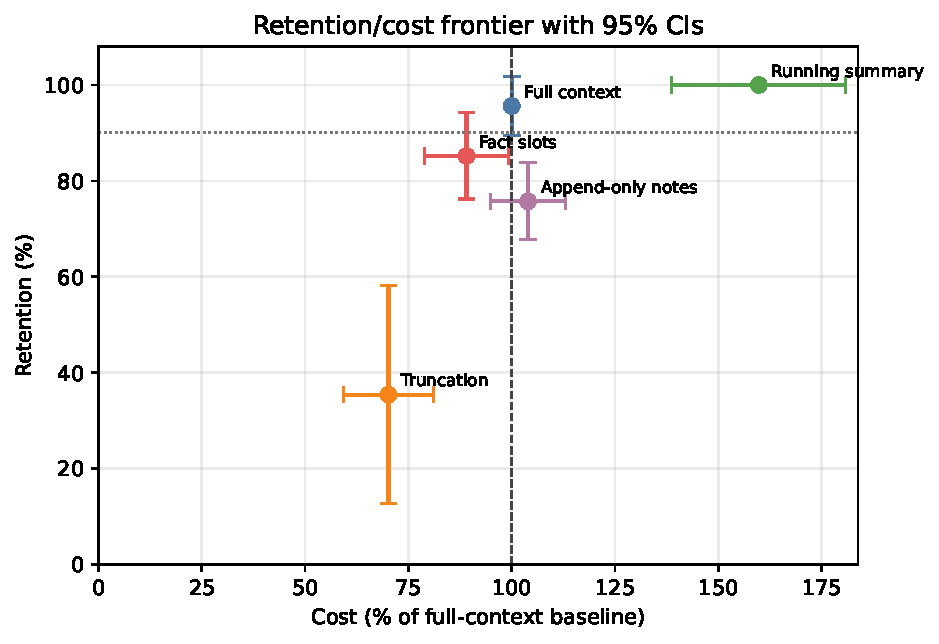
\includegraphics[width=\columnwidth]{retention_cost_frontier.pdf}
\caption{Retention/cost frontier on LoCoMo ($n=160$). Memory methods sit far to the left of full context (100\% cost) at comparable or higher retention; the slots+retrieval hybrid is on the upper-left frontier.}
\label{fig:frontier}
\end{figure}

\begin{figure}[t]
\centering
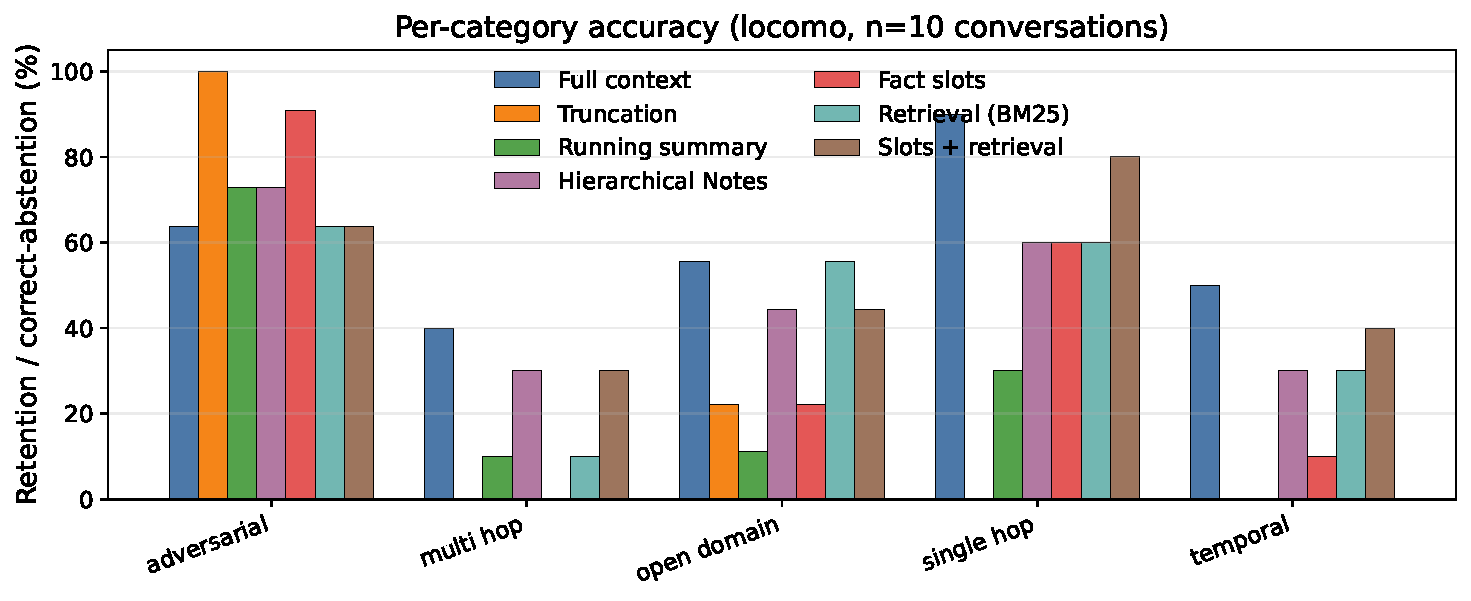
\includegraphics[width=\columnwidth]{category_retention.pdf}
\caption{Per-category accuracy on LoCoMo. Retrieval-based methods lead on single-hop, open-domain, and temporal questions; full context leads on multi-hop; low-context baselines score high on adversarial only by abstaining.}
\label{fig:category}
\end{figure}

\subsection{Statistical Power}
\label{sec:power}

Because the retrieval-vs-full-context comparison is the one we most want to make,
we quantify how underpowered it is. The paired sign test depends only on the
\emph{discordant} questions (one method correct, the other wrong). For BM25 vs.
full context there are 58 discordant pairs (36\% of $n$), 36 favoring retrieval
and 22 favoring full context ($\hat p = 0.62$); for the hybrid, 59 discordant
pairs, 36 vs. 23 ($\hat p = 0.61$). Using a normal approximation for the sign
test at $\alpha = 0.05$ two-sided and 80\% power, an effect of this size requires
about 130--160 discordant pairs, i.e.\ roughly \textbf{360--430 total questions}
at the observed $\sim$36\% discordance rate. The present $n=160$ is therefore
adequate to establish the truncation gap and the cost reduction, but not to
declare retrieval superior to full context; that claim needs the full LoCoMo
suite (or equivalently larger $n$) and is left for future work.

\subsection{Error Analysis: Why Multi-hop Fails}
\label{sec:error}

Multi-hop is the category where retrieval most clearly trails full context
(Table~\ref{tab:category}), so we analyzed all 281 LoCoMo multi-hop questions
using their gold evidence annotations. Each multi-hop question cites on average
2.6 evidence turns. Running the same BM25 retriever, the top-5 results contain on
average only \textbf{13\%} of the gold evidence turns; just 3\% of questions have
\emph{all} their evidence retrieved, while 70\% have \emph{none}. Doubling to
top-10 raises coverage only to 20\% (6\% fully covered), so the failure is
structural, not a matter of $k$. Reading 18 transcripts, the misses fall into
three recurring modes: (i) \textbf{lexical--semantic gap}---abstract questions
(``What is Caroline's identity?'', ``What does Melanie do to destress?'') share
few surface tokens with the concrete evidence (``transgender'', ``running''),
which sparse retrieval cannot bridge, including simple morphological variants
(``research'' vs.\ ``researching''); (ii) \textbf{evidence fragmentation}---
answers such as ``pottery, camping, painting, swimming'' require aggregating four
turns scattered across sessions, so a bounded top-$k$ structurally cannot supply
all of them; and (iii) \textbf{inference gap}---the answer (``single'') is implied
(``single parent'') rather than stated. Modes (i) and (iii) motivate dense or
query-rewriting retrieval; mode (ii) motivates iterative or multi-vector
retrieval. This is also why full context, which sees every turn, retains an edge
here despite its cost.

\subsection{On Fact Slots vs.\ Retrieval}
\label{sec:slots-honest}

The measured ordering is unambiguous about which lever matters most:
\textbf{BM25 retrieval is the strongest single component} on both LoCoMo and
LongMemEval.  On LoCoMo general QA (Table~\ref{tab:results}) BM25 edges the
hybrid on both cost and retention (39.4\% vs.\ 38.8\%), while latest-value fact
slots alone are the \emph{weakest} memory method (26.9\%). This pattern
persists---and sharpens---on LongMemEval's \emph{knowledge-update} category
($n=72$, Table~\ref{tab:lme_ku}), where slots should structurally excel:
because a latest-value slot table overwrites by key, it returns only the current
value when a fact changes mid-conversation, whereas append-only or retrieval
stores surface both old and new versions.

\begin{table}[h]
\centering
\caption{LongMemEval knowledge-update retention ($n=72$, LLM-judge)}
\label{tab:lme_ku}
\small
\setlength{\tabcolsep}{4pt}
\begin{tabular}{lcc}
\toprule
\textbf{Method} & \textbf{Retention} & \textbf{Cost} \\
\midrule
Full Context & 69.4\% & 100.0\% \\
Truncation & 66.7\% & 70.1\% \\
Running Summary & 47.2\% & 73.6\% \\
Hierarchical Notes & 56.9\% & 60.8\% \\
Fact-Slot Memory & 37.5\% & 59.5\% \\
Retrieval (BM25) & 73.6\% & 88.2\% \\
Slots + Retrieval & 73.6\% & 99.5\% \\
\bottomrule
\end{tabular}
\end{table}

Despite their structural advantage, fact slots alone achieve only 37.5\%
retention---the \emph{worst} of any method---because the cheap 8B extractor
fails to parse many fact updates from free-form chat.  BM25 retrieval matches
full context (73.6\% vs.\ 69.4\%, overlapping CIs) at 88\% of cost, and
truncation also tracks full context (66.7\%) because knowledge-update questions
usually reference the most recent sessions.  The slots+retrieval hybrid adds no
benefit beyond retrieval alone (73.6\% in both).  We therefore cannot claim that
fact slots help even on their intended use-case: the extractor bottleneck
outweighs the representational advantage.

We further evaluate the remaining LongMemEval categories---temporal
reasoning ($n=73$), multi-session reasoning ($n=56$), and a small
abstention probe ($n=6$)---in Tables~\ref{tab:lme_remaining}
and~\ref{tab:lme_remaining_cat}. The ordering is unchanged: the
slots+retrieval hybrid matches full context (45.2\% vs.\ 45.2\%) and BM25
retrieval nearly matches it (41.5\%; paired $\Delta=-3.7$ points,
$p=0.51$, not significant), while every memory-compression baseline and
fact slots alone fall far behind (fact slots 15.6\%, $\Delta=-29.6$
points, $p<0.001$). Per category (Table~\ref{tab:lme_remaining_cat}),
retrieval and the hybrid recover almost all of full context's temporal
accuracy (52.0\% and 49.3\% vs.\ 53.4\%), and the hybrid actually
\emph{exceeds} full context on multi-session reasoning (35.7\% vs.\
33.9\%), the hardest category, where jointly retrieving distant sessions
helps more than re-reading a long prompt. The cost savings are smaller
here---retrieval runs at 75\% of full-context cost versus 4.8\% on
LoCoMo---because LongMemEval's oracle conversations are far shorter than
LoCoMo's several-hundred-turn sessions, so there is less history for
retrieval to prune; the \emph{retention} conclusion is nonetheless
identical across both benchmarks. The abstention subset is too small
($n=6$) to support any claim beyond the familiar pattern that low-context
methods abstain more readily (Table~\ref{tab:lme_remaining_cat}).

\begin{table}[h]
\centering
\caption{LongMemEval temporal + multi-session + abstention retention ($n=135$, LLM-judge)}
\label{tab:lme_remaining}
\small
\setlength{\tabcolsep}{4pt}
\begin{tabular}{lcc}
\toprule
\textbf{Method} & \textbf{Retention} & \textbf{Cost} \\
\midrule
Full Context & 45.2\% & 100.0\% \\
Truncation & 13.3\% & 60.5\% \\
Running Summary & 16.3\% & 62.6\% \\
Hierarchical Notes & 24.4\% & 53.3\% \\
Fact-Slot Memory & 15.6\% & 51.5\% \\
Retrieval (BM25) & 41.5\% & 75.5\% \\
\textbf{Slots + Retrieval} & \textbf{45.2\%} & \textbf{85.4\%} \\
\bottomrule
\end{tabular}
\end{table}

\begin{table}[h]
\centering
\caption{Per-category retention on the remaining LongMemEval categories (\%, LLM-judge). Abstention credits correct refusal.}
\label{tab:lme_remaining_cat}
\small
\setlength{\tabcolsep}{4pt}
\begin{tabular}{lccc}
\toprule
\textbf{Method} & \textbf{Temporal} & \textbf{Multi-Sess.} & \textbf{Abstention} \\
$n$ & 73 & 56 & 6 \\
\midrule
Full Context & 53.4 & 33.9 & 50.0 \\
Truncation & 15.1 & 1.8 & 100.0 \\
Running Summary & 19.2 & 5.4 & 83.3 \\
Hierarchical Notes & 26.0 & 16.1 & 83.3 \\
Fact-Slot Memory & 13.7 & 8.9 & 100.0 \\
Retrieval (BM25) & 52.0 & 25.0 & 66.7 \\
Slots + Retrieval & 49.3 & 35.7 & 83.3 \\
\bottomrule
\end{tabular}
\end{table}

Observed properties and open hypotheses:
\begin{itemize}
    \item \textbf{Retrieval is the strongest lever on real data}: across both
    benchmarks, BM25 retrieval holds retention level with full context at a
    fraction of the cost, by surfacing query-relevant turns and avoiding
    lost-in-the-middle degradation.
    \item \textbf{Representation is secondary to extraction quality}: a cheap
    extractor that misses or misparses fact updates nullifies the structural
    advantage of latest-value slots.  An extractor-size ablation on real data
    is needed to separate the representation from the implementation.
    \item \textbf{Knowledge-update questions are mostly recent}: the proximity
    of the updated fact to the end of the conversation means truncation and
    retrieval naturally capture it, further reducing the window where slots
    could help.
    \item \textbf{Operational feasibility}: full-context prompting of real long
    conversations is rejected above a per-request token cap on a free tier, so
    compact memory is not only cheaper but sometimes the only admissible option.
    \item \textbf{Category sensitivity}: a single blended retention number hides
    large per-category differences (Table~\ref{tab:category}); abstention
    accuracy in particular must be read together with the others to avoid
    rewarding indiscriminate non-answers.
\end{itemize}

A deterministic long-horizon cost-growth simulation (cost shape only, no
retention) is provided in Appendix~\ref{app:sim} for readers interested in the
asymptotic regime beyond the lengths evaluated here.

\section{Reference Implementation}
\label{sec:implementation}

To support reproducibility, we release an open-source reference implementation of the architecture described in Algorithm~\ref{alg:hierarchical}. The implementation is a small, dependency-light Python package organized as a research repository, comprising:

\begin{itemize}
    \item \texttt{hierarchical\_memory.py} -- the core memory implementations. It includes append-only structured notes (Section~\ref{sec:notes-format}), latest-value fact slots (Section~\ref{sec:slot-format}), OpenAI-compatible provider clients, robust extraction parsing, and context builders that combine persistent memory with recent messages.
    \item \texttt{token\_utils.py} -- token-counting and reduction utilities built on \texttt{tiktoken}, implementing the Token Reduction and Cost Savings metrics of Table~\ref{tab:metrics}.
    \item \texttt{real\_datasets.py} -- adapters that load the LoCoMo and LongMemEval benchmarks into the common case/question structure, with category labels and abstention flags.
    \item \texttt{judge.py} -- the LLM-as-judge scorer using the official LongMemEval grading prompts, with a containment fallback for offline use.
    \item \texttt{evaluate.py} -- a harness that runs the seven strategies of Section~\ref{sec:baselines} over real benchmarks (and a synthetic sanity suite), with per-category metrics, per-question records, per-call failure resilience, and a \texttt{--resume} mode for rate-limited runs.
    \item \texttt{make\_figures.py} -- a deterministic artifact generator for the architecture diagram, measured-result plots, the per-category figure, and the cost-vs-length simulation.
    \item \texttt{scripts/paired\_analysis.py} and \texttt{scripts/summarize\_results.py} -- question-level paired tests (bootstrap CIs and an exact sign test) and paper-ready table extraction from the per-question records.
    \item A retained synthetic generator for offline sanity checks, pinned dependencies in \texttt{requirements.txt}, a continuous-integration smoke test, and a \texttt{README} documenting setup and usage.
\end{itemize}

The provider interface is abstracted so the small and large models can be backed by any chat-completions-compatible API; the released harness includes both an Anthropic backend and an OpenAI-compatible backend, and the evaluation in Section~\ref{sec:results} was run through the latter against the Groq inference service. Token counts are taken from the provider's own \texttt{usage} accounting rather than estimated with \texttt{tiktoken}, which is an OpenAI tokenizer and mis-counts other model families. The complete source, real-benchmark adapters, judge, raw per-question results, paired-analysis outputs, and generated figures are available at \url{https://github.com/sakul7-stack/nodemem}.

\subsection{Research Integrity and Reproducibility}

The evaluation uses openly released, human-annotated benchmarks (LoCoMo, LongMemEval) downloaded at evaluation time rather than copied into the repository or scraped from proprietary conversations. The manuscript uses original prose, avoids long quotations, and attributes related methods through the citations in the bibliography. The repository also includes a pre-submission audit script that checks unresolved placeholders, citation coverage, required result artifacts, and accidental API-key leakage. This does not certify acceptance, but it makes the empirical claims and supporting artifacts independently inspectable.

\section{Discussion}

\subsection{Limitations}

\begin{enumerate}
    \item \textbf{Partial sample}: The LoCoMo numbers are over $n=160$ questions from eight of the ten conversations; confidence intervals are wide and point estimates will shift, although the qualitative ordering is established. The LongMemEval evaluation covers knowledge-update ($n=72$) plus temporal, multi-session, and abstention ($n=135$); the abstention subset in particular ($n=6$) is too small for a firm conclusion, and the temporal/multi-session sample is drawn from the oracle setting rather than the full 500-question suite.

    \item \textbf{Absolute retention is low for all methods}: LoCoMo is hard, and a 17B synthesizer answers only about a third of questions even with full context. Our claims are therefore comparative (memory vs. full context at equal model), not about absolute accuracy; a stronger synthesizer on a paid tier would raise all rows.

    \item \textbf{Judge model}: We score with a Groq-hosted Llama judge using the LongMemEval prompts rather than GPT-4o. This keeps replication free but may differ from the canonical judge; we expose the judge as a configuration option. As a robustness check we cross-validated the \texttt{llama-3.3-70b-versatile} judge against a second, architecturally distinct judge (\texttt{gpt-oss-120b}) on a labeled 30-question subset and observed 83.3\% raw agreement (Cohen's $\kappa=0.47$, moderate-to-substantial), with neither judge showing a systematic scoring bias.

    \item \textbf{Retrieval is sparse}: The retrieval baseline is BM25 over turns. A dense-embedding backend~\cite{karpukhin2020dense} is implemented but not yet run at scale; multi-hop questions in particular may benefit from iterative or graph retrieval \cite{xu2025amem}.

    \item \textbf{Knowledge updates}: The LongMemEval knowledge-update result is in the paper but the cheap extractor's poor recall on fact updates limits the strength of any conclusion about the slot representation itself.

    \item \textbf{Tokenizer mismatch}: Cumulative token counts use \texttt{tiktoken} (OpenAI) and are approximate for Llama; real per-query counts use the provider's \texttt{usage} and are exact.

    \item \textbf{Free-tier constraints}: Per-request token caps forced the choice of a 17B synthesizer and make full-context runs slow on the longest conversations; this shapes which experiments are cheap to run but does not affect the relative metrics.
\end{enumerate}

\subsection{Future Work}

\begin{itemize}
    \item \textbf{Complete the benchmark sweep}: finish all ten LoCoMo conversations and scale the LongMemEval categories from the oracle subset to the full 500-question suite.
    \item \textbf{Dense and hybrid retrieval}: evaluate embedding-based retrieval and slot/retrieval fusion, including graph-structured memory \cite{xu2025amem, chhikara2025mem0}.
    \item \textbf{Extractor-size ablation on real data}: quantify whether the cheap 8B extractor matches a larger extractor for slot quality on LoCoMo/LongMemEval.
    \item \textbf{Stronger synthesizers}: repeat on a 70B-class or proprietary model (paid tier) to test whether the retrieval-vs-full-context ordering persists as absolute accuracy rises.
    \item \textbf{Sensitivity}: sweep \texttt{recent\_k}, segment size, slot cap, and retrieval top-$k$.
    \item \textbf{Judge robustness}: extend the two-judge cross-validation (currently 30 questions, $\kappa=0.47$) to a larger labeled subset and add GPT-4o as a third reference judge.
\end{itemize}

\section{Conclusion}

This paper evaluates cheap structured memory for LLM agents---a small model that writes latest-value fact slots, optionally fused with sparse retrieval, feeding a larger synthesizer---on \emph{real, human-annotated long conversations} rather than synthetic data. On LoCoMo with LLM-judge scoring ($n=160$ questions over conversations of several hundred turns), BM25 retrieval and a slots+retrieval hybrid cut cost to 5--9\% of full context and real input tokens by over 96\% \emph{without measurably losing} retention: their point estimates sit above full context (39.4\% and 38.8\% vs. 30.6\%) and they are significantly better than truncation ($p<0.001$), though the apparent edge over full context is only a non-significant trend ($p=0.09$--$0.12$) that a power analysis suggests needs $\approx$360--430 questions to confirm. A per-category breakdown and an error analysis localize where the methods win and lose---retrieval leads on single-hop, open-domain, and temporal questions but recovers only $\sim$13\% of gold evidence on multi-hop, where full context retains an edge. We position BM25 retrieval as the strongest single lever; fact slots are the weakest method on both general LoCoMo QA and on their intended knowledge-update use-case (37.5\% on LongMemEval), because a cheap 8B extractor misses most fact updates. We document that full-context prompting of real long conversations is operationally fragile on rate-limited tiers. These results reverse the negative finding of an earlier short, synthetic pilot: at realistic conversation lengths, cheap retrieval-based memory is a favorable point on the cost/retention frontier, with its retention parity (vs.\ full context) still to be confirmed at larger $n$. We release the harness, the real-benchmark adapters, the judge, per-question results, and the LongMemEval evaluation spanning knowledge-update, temporal, multi-session, and abstention categories; scaling from the oracle subset to the full 500-question LongMemEval suite is left for future work.

\appendices
\section{Deterministic Long-Horizon Cost Simulation}
\label{app:sim}

This appendix characterizes the cost-growth \emph{shape} at conversation lengths
beyond those evaluated live. It is a token-accounting simulation only and
\textbf{does not measure retention}; it should not be read as a quality result.
It uses a seeded generator, the same context-building code,
\texttt{tiktoken}/\texttt{cl100k} local token counts, Groq prices, deterministic
offline note extraction, and an optional note-compaction rule keeping at most 8
notes.

\begin{table}[h]
\centering
\caption{Deterministic Cost vs. Conversation Length (\% of Full Context). Cost shape only; not a retention result.}
\label{tab:growth}
\begin{tabular}{rcccc}
\toprule
\textbf{Messages} & \textbf{Trunc.} & \textbf{Hier.} & \textbf{Hier. + comp.} & \textbf{Slots} \\
\midrule
14 & 96.3\% & 121.7\% & 121.7\% & 106.2\% \\
32 & 61.4\% & 91.1\% & 91.1\% & 70.3\% \\
60 & 37.7\% & 73.3\% & 71.9\% & 47.1\% \\
120 & 20.8\% & 51.9\% & 42.3\% & 26.6\% \\
240 & 11.0\% & 42.0\% & 24.0\% & 14.0\% \\
480 & 5.7\% & 36.3\% & 13.0\% & 7.4\% \\
\bottomrule
\end{tabular}
\end{table}

The simulation shows the expected divergence: append-only notes fall below full
context after a short warm-up but remain well above truncation, while bounded
notes and fact slots track close to truncation by 480 messages. This motivates
bounded memory at long horizons but, again, says nothing about whether the
bounded memory still answers correctly---the live retention experiments above are
the load-bearing evidence.

\section*{Acknowledgment}

The authors thank Tribhuvan University and the Institute of Engineering for academic support. This research was conducted independently without external funding.

\begin{thebibliography}{99}

\bibitem{packer2023memgpt}
C. Packer, S. Wooders, K. Lin, V. Fang, S. G. Patil, I. Stoica, and J. E. Gonzalez, ``MemGPT: Towards LLMs as operating systems,'' \textit{arXiv preprint arXiv:2310.08560}, 2023.

\bibitem{jiang2023llmlingua}
H. Jiang, Q. Wu, C.-Y. Lin, Y. Yang, and L. Qiu, ``LLMLingua: Compressing prompts for accelerated inference of large language models,'' in \textit{Proc. Conf. Empirical Methods in Natural Language Processing (EMNLP)}, 2023, pp. 13358--13376.

\bibitem{nfliu2023lost}
N. F. Liu, K. Lin, J. Hewitt, A. Paranjape, M. Bevilacqua, F. Petroni, and P. Liang, ``Lost in the middle: How language models use long contexts,'' \textit{Trans. Assoc. Comput. Linguistics (TACL)}, vol. 12, pp. 157--173, 2024.

\bibitem{zhang2024memorysurvey}
Z. Zhang, X. Bo, C. Ma, R. Li, X. Chen, Q. Dai, J. Zhu, Z. Dong, and J.-R. Wen, ``A survey on the memory mechanism of large language model based agents,'' \textit{ACM Trans. Inf. Syst.}, 2024. (Also \textit{arXiv preprint arXiv:2404.13501}.)

\bibitem{acl2024}
M. Sung, S. Lee, J. Kim, and S. Kim, ``Context-aware LLM translation system using conversation summarization and dialogue history,'' in \textit{Proc. 9th Conf. Machine Translation (WMT)}, 2024, pp. 1011--1015.

\bibitem{park2023generative}
J. S. Park et al., ``Generative agents: Interactive simulacra of human behavior,'' in \textit{Proc. 36th Annual ACM Symposium on User Interface Software and Technology (UIST)}, 2023, pp. 1--22.

\bibitem{shinn2023reflexion}
N. Shinn et al., ``Reflexion: Language agents with verbal reinforcement learning,'' in \textit{Advances in Neural Information Processing Systems (NeurIPS)}, vol. 36, 2023.

\bibitem{zhou2024agents}
S. Zhou et al., ``WebArena: A realistic web environment for building autonomous agents,'' in \textit{Proc. International Conference on Learning Representations (ICLR)}, 2024.

\bibitem{chen2023frugalgpt}
L. Chen et al., ``FrugalGPT: How to use large language models while reducing cost and improving performance,'' \textit{arXiv preprint arXiv:2305.05176}, 2023.

\bibitem{zhong2024memorybank}
W. Zhong et al., ``MemoryBank: Enhancing large language models with long-term memory,'' in \textit{Proc. AAAI Conference on Artificial Intelligence}, 2024.

\bibitem{bang2023gptcache}
F. Bang, ``GPTCache: An open-source semantic cache for LLM applications enabling faster answers and cost savings,'' in \textit{Proc. 3rd Workshop for Natural Language Processing Open Source Software (NLP-OSS)}, 2023, pp. 212--218.

\bibitem{karpukhin2020dense}
V. Karpukhin et al., ``Dense passage retrieval for open-domain question answering,'' in \textit{Proc. Conference on Empirical Methods in Natural Language Processing (EMNLP)}, 2020, pp. 6769--6781.

\bibitem{maharana2024locomo}
A. Maharana, D.-H. Lee, S. Tulyakov, M. Bansal, F. Barbieri, and Y. Fang, ``Evaluating very long-term conversational memory of LLM agents,'' in \textit{Proc. 62nd Annual Meeting of the Association for Computational Linguistics (ACL)}, 2024.

\bibitem{wu2024longmemeval}
D. Wu, H. Wang, W. Yu, Y. Zhang, K.-W. Chang, and D. Yu, ``LongMemEval: Benchmarking chat assistants on long-term interactive memory,'' in \textit{Proc. International Conference on Learning Representations (ICLR)}, 2025. (arXiv:2410.10813.)

\bibitem{chhikara2025mem0}
P. Chhikara, D. Khant, S. Aryan, T. Singh, and D. Yadav, ``Mem0: Building production-ready AI agents with scalable long-term memory,'' \textit{arXiv preprint arXiv:2504.19413}, 2025.

\bibitem{xu2025amem}
W. Xu, Z. Liang, K. Mei, H. Gao, J. Tan, and Y. Zhang, ``A-MEM: Agentic memory for LLM agents,'' in \textit{Advances in Neural Information Processing Systems (NeurIPS)}, 2025. (arXiv:2502.12110.)

\end{thebibliography}

\end{document}